
%% bare_conf.tex
%% V1.3
%% 2007/01/11
%% by Michael Shell
%% See:
%% http://www.michaelshell.org/
%% for current contact information.
%%
%% This is a skeleton file demonstrating the use of IEEEtran.cls
%% (requires IEEEtran.cls version 1.7 or later) with an IEEE conference paper.
%%
%% Support sites:
%% http://www.michaelshell.org/tex/ieeetran/
%% http://www.ctan.org/tex-archive/macros/latex/contrib/IEEEtran/
%% and
%% http://www.ieee.org/

%%*************************************************************************
%% Legal Notice:
%% This code is offered as-is without any warranty either expressed or
%% implied; without even the implied warranty of MERCHANTABILITY or
%% FITNESS FOR A PARTICULAR PURPOSE! 
%% User assumes all risk.
%% In no event shall IEEE or any contributor to this code be liable for
%% any damages or losses, including, but not limited to, incidental,
%% consequential, or any other damages, resulting from the use or misuse
%% of any information contained here.
%%
%% All comments are the opinions of their respective authors and are not
%% necessarily endorsed by the IEEE.
%%
%% This work is distributed under the LaTeX Project Public License (LPPL)
%% ( http://www.latex-project.org/ ) version 1.3, and may be freely used,
%% distributed and modified. A copy of the LPPL, version 1.3, is included
%% in the base LaTeX documentation of all distributions of LaTeX released
%% 2003/12/01 or later.
%% Retain all contribution notices and credits.
%% ** Modified files should be clearly indicated as such, including  **
%% ** renaming them and changing author support contact information. **
%%
%% File list of work: IEEEtran.cls, IEEEtran_HOWTO.pdf, bare_adv.tex,
%%                    bare_conf.tex, bare_jrnl.tex, bare_jrnl_compsoc.tex
%%*************************************************************************

% *** Authors should verify (and, if needed, correct) their LaTeX system  ***
% *** with the testflow diagnostic prior to trusting their LaTeX platform ***
% *** with production work. IEEE's font choices can trigger bugs that do  ***
% *** not appear when using other class files.                            ***
% The testflow support page is at:
% http://www.michaelshell.org/tex/testflow/



% Note that the a4paper option is mainly intended so that authors in
% countries using A4 can easily print to A4 and see how their papers will
% look in print - the typesetting of the document will not typically be
% affected with changes in paper size (but the bottom and side margins will).
% Use the testflow package mentioned above to verify correct handling of
% both paper sizes by the user's LaTeX system.
%
% Also note that the "draftcls" or "draftclsnofoot", not "draft", option
% should be used if it is desired that the figures are to be displayed in
% draft mode.
%
\documentclass[conference]{IEEEtran}
\usepackage{blindtext, graphicx, amsmath}

% table config
\usepackage{subfig}
\captionsetup[table]{belowskip=10pt,aboveskip=10pt}
\usepackage{colortbl}
\definecolor{Gray}{gray}{0.7}

% correct bad hyphenation here
\hyphenation{op-tical net-works semi-conduc-tor}

\usepackage{hyperref}
\usepackage{mathpazo}

\begin{document}

%
% paper title
% can use linebreaks \\ within to get better formatting as desired
\title{Batik Classification using Deep Convolutional Network Transfer Learning}


% author names and affiliations
% use a multiple column layout for up to three different
% affiliations
\author{

\IEEEauthorblockN{Yohanes Gultom}
\IEEEauthorblockA{Faculty of Computer Science\\
University of Indonesia\\
yohanes.gultom@ui.ac.id}
\and
\IEEEauthorblockN{Aniati Murni Arymurthy}
\IEEEauthorblockA{Faculty of Computer Science\\
University of Indonesia\\
aniati@cs.ui.ac.id}

}

% make the title area
\maketitle


\begin{abstract}
Batik fabric is one of the most profound cultural heritage in Indonesia. Hence, continuous research on understanding it is necessary to preserve it. Despite of being one of the most common research task, Batik's pattern automatic classification still requires some improvement especially in regards to invariance dilemma. Convolutional neural network (ConvNet) is one of deep learning architecture which able to learn data representation by combining local receptive inputs, weight sharing and convolutions in order to solve invariance dilemma in image classification. Our experiments showed that the proposed model, which used deep ConvNet VGG16 for transfer learning, outperformed SIFT-based and SURF-based classification models in both accuracy and speed. Our model achieved 74\% accuracy and required 64s processing time (with GPU) while SIFT and SURF achieved 25\% (in 492s) and 40\% (in 416s) respectively. 
\end{abstract}

\begin{IEEEkeywords}
Batik, classification, deep learning, transfer learning
\end{IEEEkeywords}

\section{Introduction}

Batik fabric is one of the most profound cultural heritage in Indonesia. Hence, continuous research on understanding it is necessary to preserve it. One of the most popular research topic is batik classification.

Since the most prominent feature of Batik is its uniquely recurring pattern (motifs), it's natural to consider it as a key to classification. To be more specific, recognition of Batik's motifs has been considered as one of the most successful technique in Batik classification especially using Scale-Invariant Feature Transform (SIFT) \cite{azhar2015batik} \cite{nurhaida2015automatic} and Speeded up robust features (SURF) \cite{willy2013evaluation}. Classifications using other features such as color and contrast are showing potentials but need to be researched further \cite{moertini2005algorithms}.

Deep learning based models have outperformed state-of-the-art methods in many domains including image classification and object recognition \cite{lecun2015deep}. One of the deep learning models, convolutional neural network (convnet) \cite{lecun1998gradient}, is currently considered as the state-of-the-art of image classification model as it was used as the base structure by ILSVRC-2014 top achievers \cite{simonyan2014very}. Therefore convnet may also be used to improve result on other image classification problems such as Batik classification.

In this paper, a deep learning model is proposed as a better alternative to classify most common Batif motifs: Parang, Lereng, Kawung, Ceplok and Nitik. VGG16 deep convnet pretrained model \cite{simonyan2014very} is used as first part of the model to automatically extract features from images and a fully-connected neural network is trained and used as classifier. The proposed model is compared with two SVM classifiers with different hand-crafted feature extractor, SIFT and SURF.

\section{Related Works}

\begin{figure}[!b]
\centering
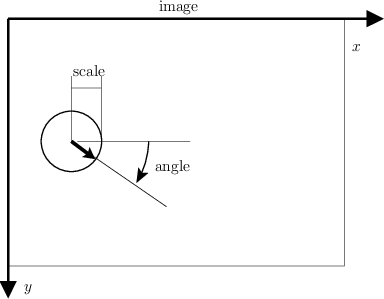
\includegraphics[width=2.0in]{sift-keypoint}
\caption{SIFT Keypoint}
\label{fig_keypoint}
\end{figure}

\begin{figure}[!b]
\centering
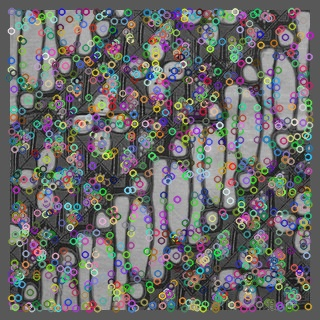
\includegraphics[width=2.0in]{batik-parang-keypoints}
\caption{SIFT keypoints in Batik Parang}
\label{fig_batik_parang_keypoints}
\end{figure}

%\begin{figure}[!b]
%\centering
%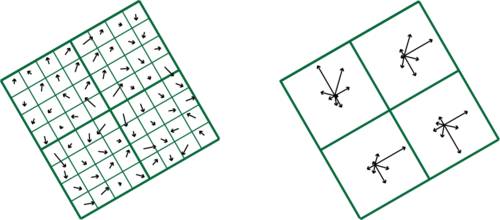
\includegraphics[width=2.0in]{sift-descriptor-1}
%\caption{SIFT descriptor}
%\label{fig_sift_descriptor_1}
%\end{figure}

Recent researches in Batik classification can be divided into two groups: (1) Researches on classification using handcrafted features (eg. SIFT and SURF), and (2) researches on classification using automatically extracted features using deep learning.

\subsection{Classification using Handcrafted Features}

\begin{figure}[!t]
\centering
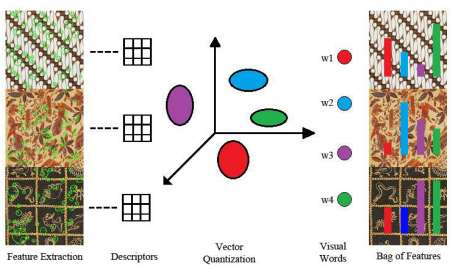
\includegraphics[width=3.0in]{sift-bag-of-words}
\caption{SIFT for building bag of words visual vocabularies}
\label{fig_sift_bag_of_words}
\end{figure}

Since Batik classification has been researched for quite some time, current available methods are robust enough to noise addition, compression, and retouching of the input images. However most of them are still having difficulties with variance in transformations which involve either translation, rotation, scaling or combinations of them \cite{nurhaida2015automatic}. Recent improvements on Batik classification were motivated by the emergence of Scale-Invariant Feature Transform (SIFT)\cite{lowe2004distinctive} and Speeded up robust features (SURF)\cite{bay2006surf}. Both of these keypoint-based feature extraction methods are proposed to solve the transformation invariance dilemma.

SIFT keypoint is a circular image region with an orientation which can be obtained by detecting extrema of Difference of Gaussian (DoG) pyramid \cite{lowe2004distinctive}. It's defined by four parameters: center coordinates x and y, scale and its orientation (an angle expressed in radians) as shown in Figure \ref{fig_keypoint}. An image, for example Batik image, may contains multiple keypoints as shown in Figure \ref{fig_keypoint}. In order to be efficiently and effectively used as a feature for classification, the keypoint need to be represented as SIFT descriptor. By definition it is a 3-dimensional spatial histogram of the image gradients characterizing a SIFT keypoint.

Recent research \cite{nurhaida2015automatic} proved that using SIFT descriptors to calculate similarity between Batik images can give 91.53\% accuracy. Voting Hough Transform was applied to the descriptors to eliminate mismatched keypoint candidates. This research suggested that the original SIFT descriptor matching shouldn't be directly used to calculate similarity of Batik images due to many numbers of mismatched keypoints. The method used in this research is described by diagram in Figure \ref{fig_sift_hough_voting_method}.

Another research \cite{azhar2015batik} proposed a classification method using support vector machine (SVM) fed by bag of words (BOF) features extracted using SIFT descriptors as described by Figure \ref{fig_songket_sift_vs_surf_methodology}. In this research, SIFT descriptors also weren't used directly as features for SVM but were clustered using k-means vector quantization algorithm to build vocabularies. These visual vocabularies then used to describe each images and fed to SVM classifier. The experiment results showed very good average accuracy of 97.67\% for normal images, 95.47\% for rotated images and 79\% for scaled images. Besides that SIFT and bag of words made a good feature extractor, this research also concludes that further works need to handle scaled Batik image cases.

An earlier research \cite{willy2013evaluation} proved that SURF can extract transformation invariant features faster than SIFT for classification of Songket, another Indonesian traditional fabric with motifs just like Batik. Unlike the others, this research used SIFT and SURF features directly to compute the matching scores between Songket images. The scores are calculated by (1) the number of matched keypoints and (2) the average total distance of the n-nearest keypoints as shown in Figure \ref{fig_songket_sift_vs_surf_methodology}. The result of experiments showed that the matching accuracy with SIFT features was 92-100\% and 65-97\% with SURF. With SURF features, the accuracy dropped quite significant if salt and pepper noises were added while SIFT was more stable. Apparently, this one wasn't paying much attention to transformation variance as it didn't apply transformation noise as in other research\cite{azhar2015batik}.

\begin{figure}[!b]
\centering
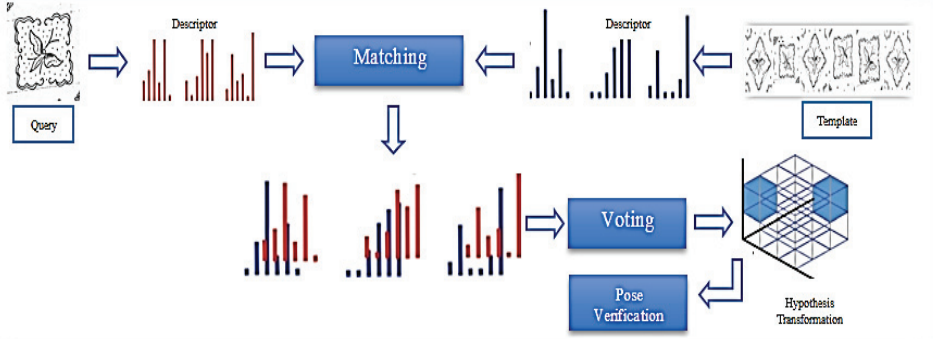
\includegraphics[width=3.0in]{sift-hough-voting-method}
\caption{SIFT with Hough voting method for Batik classification}
\label{fig_sift_hough_voting_method}
\end{figure}

\begin{figure}[!b]
\centering
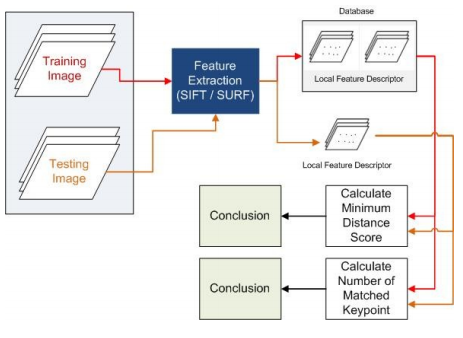
\includegraphics[width=3.0in]{songket-sift-vs-surf-methodology}
\caption{SIFT vs SURF method for Songket classification}
\label{fig_songket_sift_vs_surf_methodology}
\end{figure}

\subsection{Classification using Deep Learning}

Deep learning is a multilayer representation learning in artificial neural network \cite{lecun2015deep}. While representation learning itself is a method in machine learning to automatically extract/learn representation (features) from raw data. The representation of the raw data then can be used for recognition or classification task. Some fundamental deep learning architectures for instances are convolutional neural network (ConvNet), deep belief network (DBN), autoencoder (AE) and recurrent neural network (RNN). Despite of being an old idea, it was recently emerged due to the several factors: (1) discovery of new techniques (eg. pretraining \& dropout) and new activation functions (eg. ReLU), (2) enormous supply of data (big data), and (3) rapid improvement in computational hardware, especially GPU.

Although not yet many, the advent of deep learning also motivated a research on Batik classification using convolutional stacked autoencoder \cite{menzata2014sistem}. This research proposed the usage of convolutional transformations to reduce the input nodes of stacked autoencoder. The experiment showed that this deep architecture was able to achieve 81,73\% accuracy by using small patches of Batik for training. When noises were added its accuracy dropped to 49\% for gaussian noises, 61\% for rotations, 70\% for scalings and 75\% for illumination noises. Another research have shown that deep architecture such as convolutional neural network should be able to outperform handcrafted features such as SIFT\cite{fischer2014descriptor}. Therefore further research on Batik classification using deep learning architectures is encouraged.

\section{Methodology}

We propose a deep convolutional neural network composed by a pre-trained VGG16 (without its top layer) as automatic feature extractor and a fully-connected feed-forward neural network as classifier. The method of using pre-trained deep network as part of another neural network to solve different (but related) task can be considered as transfer learning or self-taught learning \cite{raina2007self}.

\begin{figure}[!t]
\centering
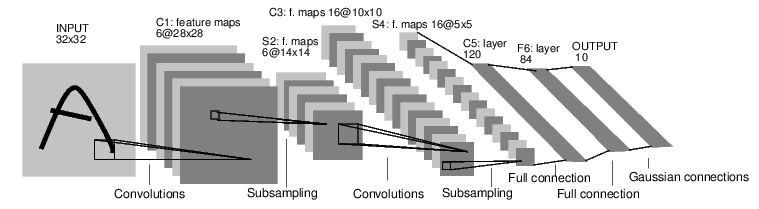
\includegraphics[width=3.0in]{lenet5}
\caption{LeNet5 convolutional network}
\label{fig_lenet5_convnet}
\end{figure}


\begin{figure}[!t]
\centering
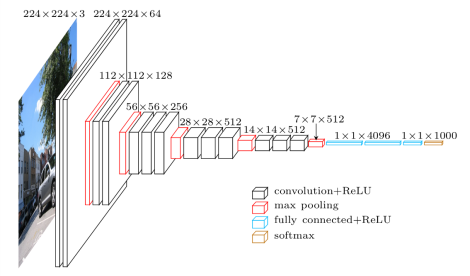
\includegraphics[width=3.0in]{vgg16}
\caption{VGG16 deep convolutional network model of Visual Geometry Group, Oxford}
\label{fig_vgg16}
\end{figure}

\subsection{Convolutional Neural Network}

Convolutional network is a special kind of neural network optimized to learn representation of an image \cite{lecun2015deep}. It introduces 2 new types of hidden layers: convolutional and subsampling/pooling layers. Each layer in convnet connects neurons (pixels) from their input layer in form of local receptives (square patches) through a shared weights to a feature map \cite{lecun1998gradient}. On top of a set of convolutional and pooling layers, some fully-connected layers are added as classifier as described by Figure \ref{fig_lenet5_convnet}.

Our proposed model uses 5 set of convolutional and pooling layers using rectified unit (ReLu) activation function following example of VGG16 as shown in Figure \ref{fig_vgg16}. The differences are our model uses 2 fully-connected hyperbolic tangent (tanh) (Equation \ref{eq_tanh}) activated layers as classifier (instead of ReLu) and a SoftMax (Equation \ref{eq_softmax}) layer as an output. We also uses Dropout regularization after each tanh fully-connected layers to avoid overfitting by randomly drop/turn off (set value to zero) hidden nodes (Equation \ref{eq_dropout}) \cite{srivastava2014dropout}.

\begin{equation}
y_{i}={\frac {2}{1+e^{-2x _{i}}}}-1
\label{eq_tanh}
\end{equation}

%\begin{equation}
%f(x)=\left\{{\begin{array}{rcl}0&{\mbox{for}}&x<0\\x&{\mbox{for}}&x\geq 0\end{array}}\right.
%\label{eq_relu}
%\end{equation}

\begin{equation}
y_{i}={\frac {e^{x _{i}}}{\sum _{k=1}^K e^{x _{k}}}} \quad \text{, for i=1..K}
\label{eq_softmax}
\end{equation}

\begin{align}
r_{j}^{x} \sim Bernoulli(p), \nonumber \\
\tilde{y} _{i}= r _{i} * y _{i}
\label{eq_dropout}
\end{align}

\subsection{Transfer Learning}

Deep neural networks usually requires a lot of training data in order to learn the representation of the data. In case there is not enough training data, there are several techniques to help neural networks model learns data representation using small training data. One of the technique is transferring knowledge of other pre-trained neural network model to our model. This technique is known as transfer learning or self-taught learning \cite{raina2007self}.

Our proposed model uses transferred knowledge (layer weights) from pre-trained VGG16 model provided by deep learning framework Keras \footnote{\url{https://keras.io/applications/\#vgg16}} which was pre-trained using 1,000,000 images dataset from ImageNet. We use VGG16 bottom layers weights (excluding the fully-connected layers) to initialize our model weights and train the classifier part only. This method allows us to shorten the time needed to train our model. Moreover, training the model using GPU improve the speed even more.

To improve comprehension and reproducibility, we also publish our model Python code in public online code repository\footnote{\url{https://github.com/yohanesgultom/deep-learning-batik-classification}}. We use opensource Theano-backed Keras as deep learning framework and Scikit-Learn\footnote{\url{http://scikit-learn.org/}} as model evaluation framework.

\section{Experiments and Results}

In order to measure the performance of our model, we trained our model and compared it with SIFT and SURF based models.

\subsection{Experiments}

The dataset was used in this research is a Batik dataset compiled by Machine Learning and Computer Vision (MLCV) Lab, Faculty of Computer Science, University of Indonesia. This dataset consists of 603 Batik photos ($\pm$ 78.3 MB) gathered from various sources thus having different size, quality and view angle.

We also tried to tune the dataset by deleting some duplicated (similar photos under a class) and conflicting photos (same photos exist under different classes). The tuned dataset has 523 photos left ($\pm$ 68.7 MB) and considered as separate dataset in this experiment.

All classifiers in this experiment were trained using 553 Batik photos (around 52-169 per class) and tested using 50 photos (10 classes per class) from regular dataset (9:1 ratio). The classifiers were also trained using 476 photos and tested with 47 photos from tuned dataset in order to observe the difference.

Our neural network classifier was trained for 50 epoch using Cross Entropy function to calculate loss (Equation \ref{eq_cross_entropy_loss}) and optimized using Stochastic Gradient Descent (SGD) (Equation \ref{eq_sgd}) to update weights.

\begin{equation}
V(f(\vec{x}),t) = -t\ln(f(\vec{x}))-(1-t)\ln(1-f(\vec{x}))
\label{eq_cross_entropy_loss}
\end{equation}

\begin{equation}
w:=w-\eta \nabla Q_{i}(w)+\alpha \Delta w
\label{eq_sgd}
\end{equation}

The SIFT and SURF models were trained in similar manner using similar methods described in related research \cite{azhar2015batik} and also illustrated in Figure \ref{fig_sift_bag_of_words}:
\begin{enumerate}
\item Image descriptors were extracted according to their feature extractor (SIFT or SURF)
\item Descriptors were clustered to 5 clusters using K-Means to get visual vocabularies for Bag of Words (BoW)
\item Those 5 visual vocabularies then used to compute BoW features from SIFT/SURF image descriptors
\item Finally a multi-class SVM classifier were trained using the BoW features
\end{enumerate}

All experiments were conducted using Intel Core i7-5960X CPU, 32 GB RAM, NVIDIA GTX 1080 8GB GPU, 240GB SSD, Debian 8 OS. The proposed model ran on GPU while SIFT/SURF SVM models ran on CPU as there were yet mature GPU implementation of the algorithms.

\subsection{Results}

As shown in Figure \ref{fig_accuracy_comparison}, the proposed model outperformed SIFT and SURF based classifier by 24\% and 34\% respectively when using regular dataset. Moreover by using tuned dataset, our model outperformed other models by larger margin 34\% and 49\%.

Parallel execution of the proposed model in GPU made the total processing time (feature extraction, training and testing) much shorter than other models which ran on single CPU. As described in Figure \ref{fig_time_comparison}, our model only requires 10-12\% of SIFT/SURF processing time.

\begin{table*}
\centering
\renewcommand{\arraystretch}{1.5}
\begin{tabular}{|p{5cm}|c|c|c|c|}
\rowcolor{Gray}
\hline \centering \textbf{Method} & \textbf{Accuracy} & \textbf{Accuracy (Tuned Dataset)}  & \textbf{Time} & \textbf{Time (Tuned Dataset)} \\ 
\hline SIFT + Bag of Words + SVM  & 0.22 & 0.25 & 554  & 492 \\ 
\hline SURF + Bag of Words + SVM  & 0.32 & 0.40 & 696 & 616 \\ 
\hline VGG16 + Neural Network & 0.56 & 0.74 & 72 & 64 \\ 
\hline 
\end{tabular}
\caption{Experiment results showed that the proposed model outperformed SIFT and SURF based models in term of accuracy and processing time}
\label{tab_experiment_results}
\end{table*}

\begin{figure}
\centering
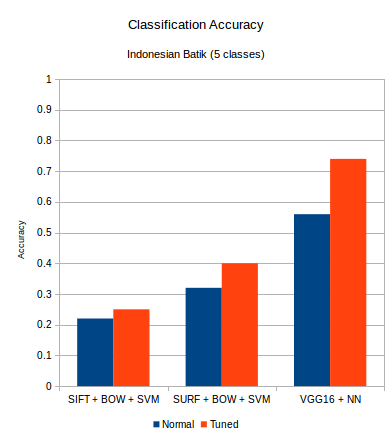
\includegraphics[width=3.0in]{chart_accuracy}
\caption{Models accuracy comparison}
\label{fig_accuracy_comparison}
\end{figure}


\begin{figure}
\centering
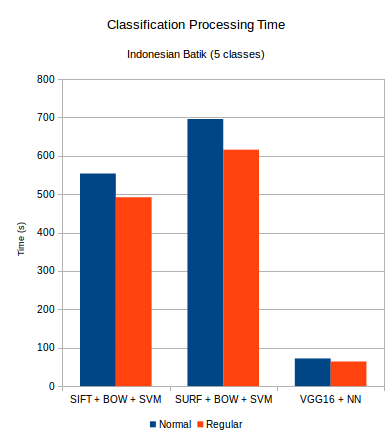
\includegraphics[width=3.0in]{chart_time}
\caption{Execution (from preprocessing to classification) time comparison}
\label{fig_time_comparison}
\end{figure}


\section{Conclusion and Future Works}

As shown by the experiments, our model, which is based on deep convolutional network, outperformed SIFT and SURF based models in term of accuracy as well as processing time. This confirms that automatic feature extraction using pre-trained convolutional are able to handle transformation invariant features such as Batik motifs better than SIFT and SURF as also concluded by related research \cite{fischer2014descriptor}.

Moreover, deep neural networks is more scalable as its training computation is composed of matrix multiplication which can be easily parallelized on GPU. Supported by keep-growing GPU hardwares, deep neural networks can always be improved in term of speed and capacity.

We also found out that current Batik dataset has a lot of room for improvements:

\begin{enumerate}
\item \textbf{Multi-labeled data}. As majority of the data are mixed-motif Batik, the dataset must provide more than one labels for each applicable sample.
\item \textbf{Clearly distinguished samples between classes}. For instance, Parang and Lereng motifs data often overlaps each other. This condition often confuses classifier during training and causes less accurate generalization.
\item \textbf{Homogeneous quality of data}. Due to the various sources of data, the quality (resolution, size, view angle) of the data are also various. Removing low quality data and preprocessing high quality ones may produce homogeneous data and improve classifier training process.
\end{enumerate}

% Can use something like this to put references on a page
% by themselves when using endfloat and the captionsoff option.
\ifCLASSOPTIONcaptionsoff
  \newpage
\fi

\bibliography{laporan}
\bibliographystyle{IEEEtran}

% that's all folks
\end{document}


